\chapter{Results}
\label{sec:results}

Comparing the lineplot of page views from 2009 as shown in the paper by Yasseri et al. (Figure 1) to the lineplot recreated in Figure \ref{fig:figure1} of this report, it is evident that the two lineplots exhibit close similarity. The peak in page views aligns with the date of the 2009 European Parliament Elections, indicating a clear correlation between the election and the increased interest in related Wikipedia articles. 
\begin{figure*}[]
    \centering
    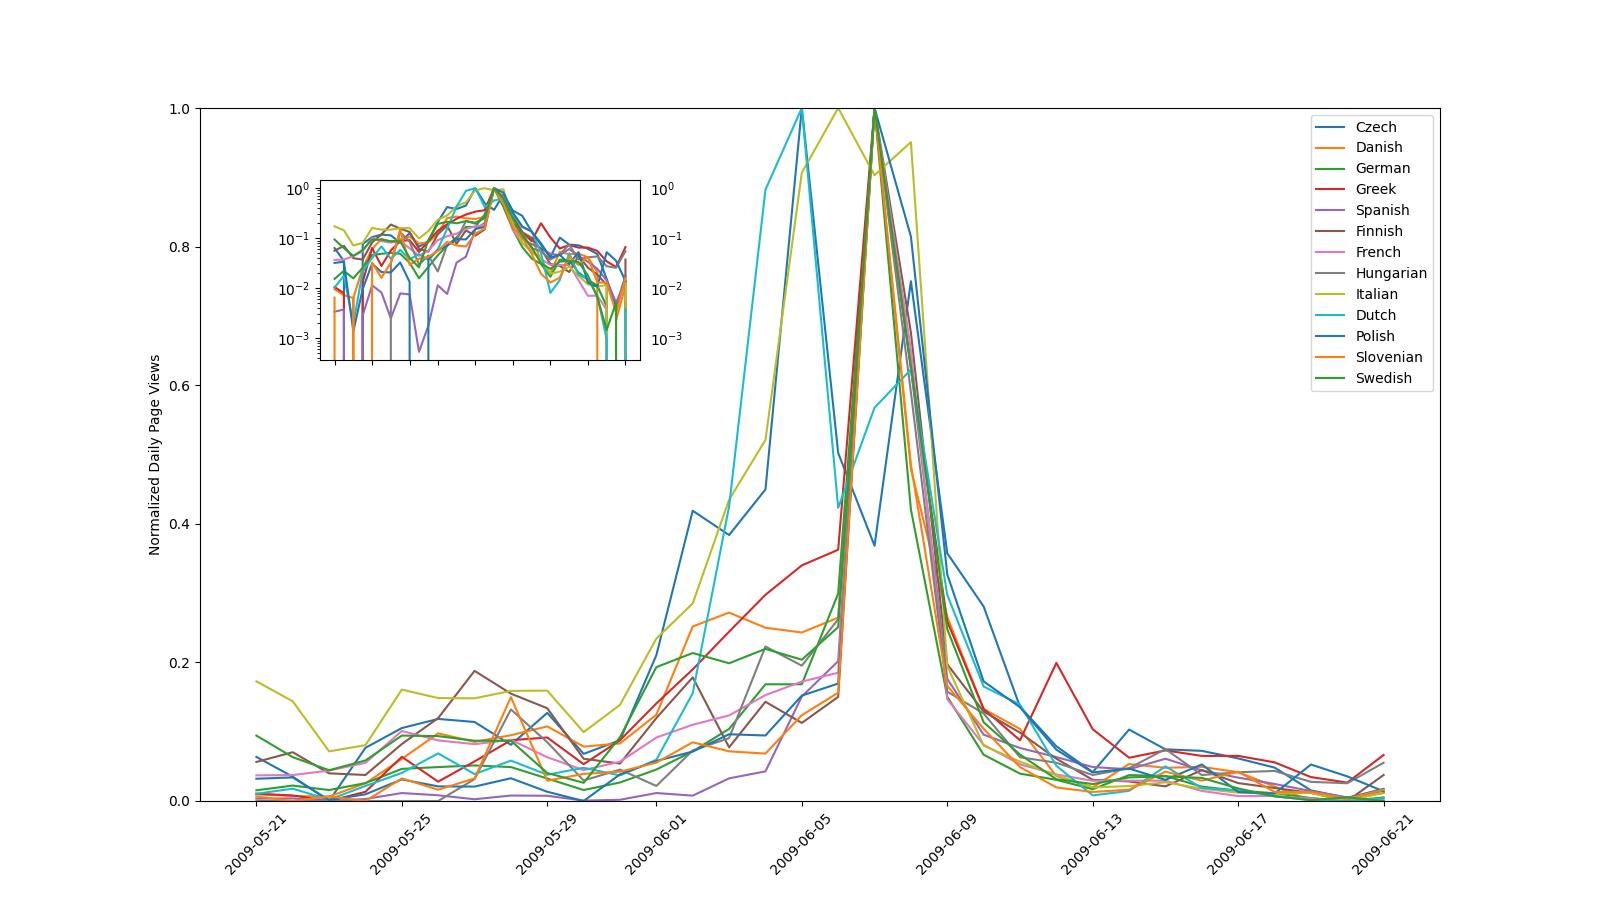
\includegraphics[width=\textwidth]{fig/lineplot_2009.png}
    \caption{'Normalized Wikipedia Election Page Views two weeks before and after the 2009 European Parliament Elections'}
    \label{fig:figure1}
\end{figure*} 
However, when visualizing the data from 2014 and 2019 in the same way, it becomes apparent that the patterns differ from those observed in the 2009 data. The peaks and fluctuations in page views do not align as closely with the election dates in these years. 
\begin{figure*}[t!]
    \centering
    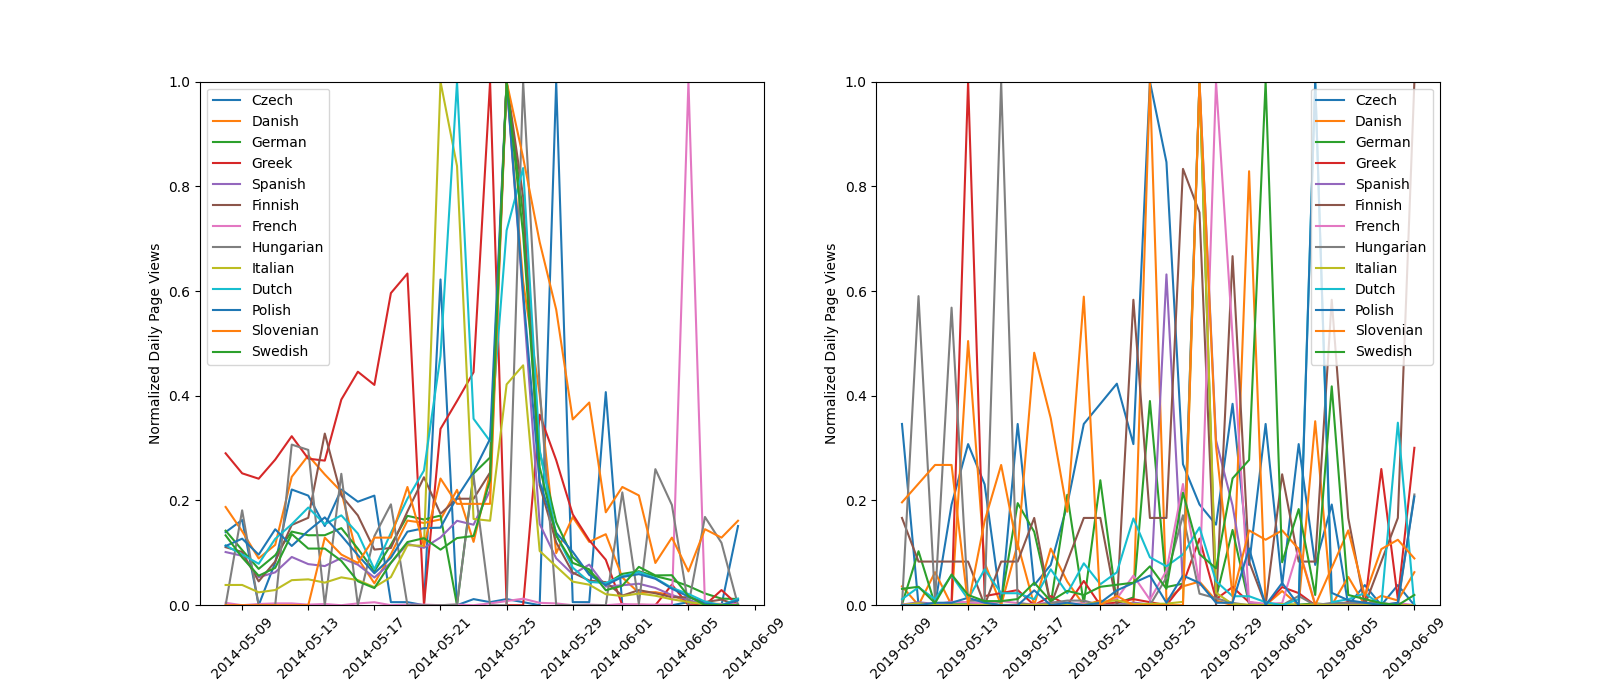
\includegraphics[width=\textwidth]{fig/lineplot_2014_2019.png}
    \caption{'Normalized Wikipedia Election Page Views two weeks before and after the 2014 (left) and 2019 (right) European Parliament Elections'}
    \label{fig:figure2}
\end{figure*}

Taking a closer look at the values of Hungary, a country  where the peak does not correspond to the election date, it becomes apparent that there could be errors in the data or its retrieval, as page views are at around zero after three seemingly random peaks till the 15th of June. Further analysis has to be performed under the assumption that the data is erroneous.

The correlation analysis conducted on the relative changes of page views and turnout from 2009 to 2014 and from 2014 to 2019 did not yield statistically significant results. For the time period of 2009 to 2014, the correlation coefficient was calculated to be -0.2884. However, with a p-value of 0.3392, the correlation is not statistically significant. Similarly, for the time period of 2014 to 2019, the correlation coefficient was found to be 0.3662. However, the corresponding p-value of 0.2184 suggests that this correlation is also not statistically significant. Based on these findings, there is no strong evidence to support a significant correlation between the relative changes in page views and turnout during these time periods.

\begin{figure*}[]
    \centering
    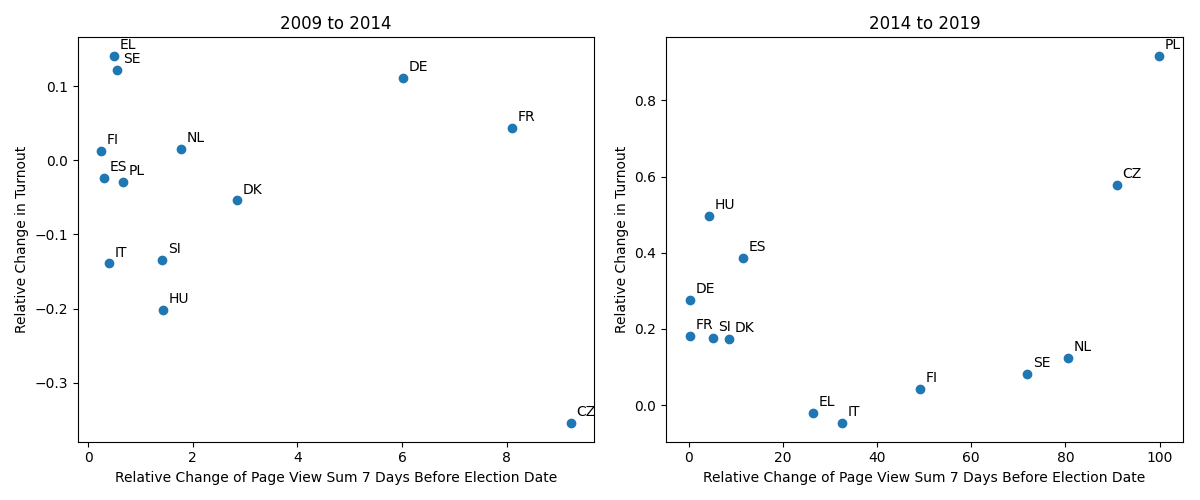
\includegraphics[width=\textwidth]{fig/scatter.png}
    \caption{"Scatterplot of Relative Changes in Page Views and Turnout"}
    \label{fig:figure4}
\end{figure*}

This is supported by visualizing the respective relative changes in a scatter plot visible in Figure \ref{fig:figure4}.